\begin{figure}[p!]
    \centering
    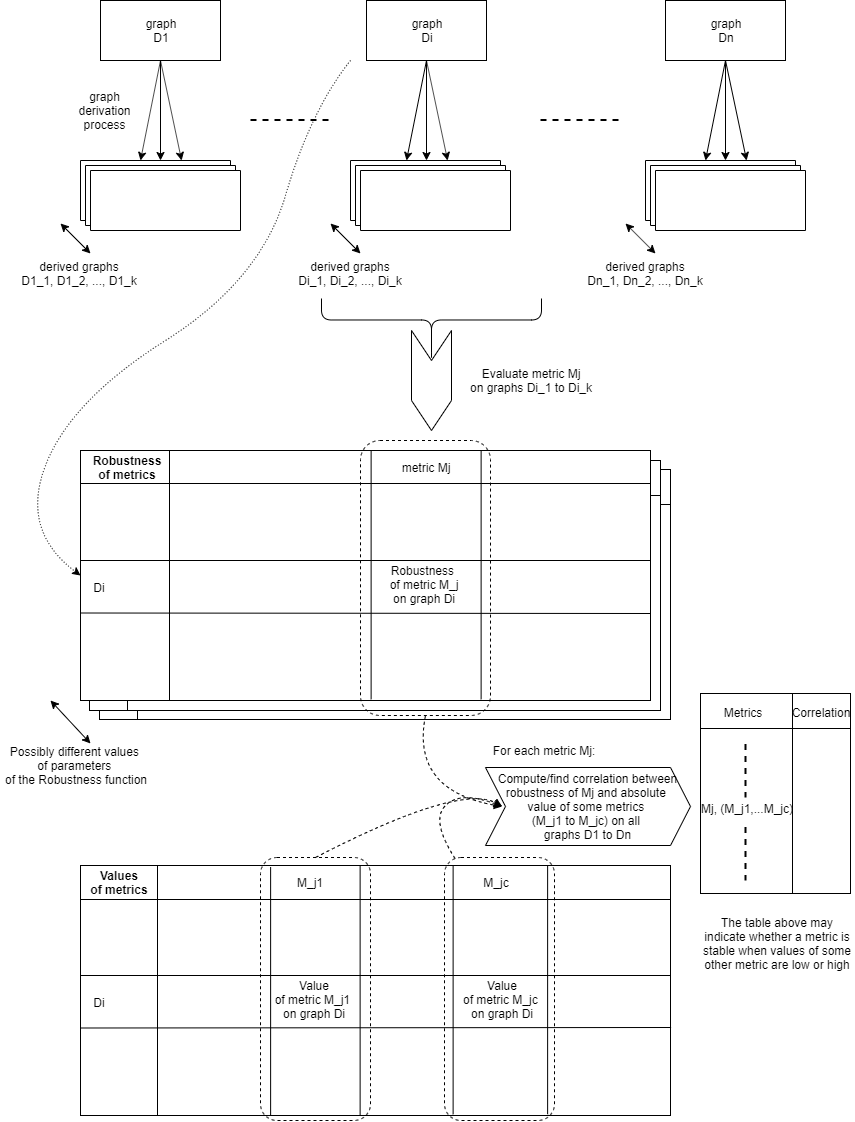
\includegraphics[width=15.5cm]{proposal_diagram1.png}
    \caption{An illustration of the evaluation process.
    A generator is used to generate perturbed graphs from each input dataset.
    Each metric from a chosen set of metrics is evaluated on all petrurbed graphs.
    From those results, robustness values of each metric on each dataset are calculated using each chosen robustness measures.
    This is referred to in the project as the ``Main pipeline''}
    \label{fig:overview_prop_diagram}
    \todo{make this diagram up to date, using notation from~\nameref{ch:preparation}}
\end{figure}
